\documentclass{article}
\usepackage{graphicx} % Required for inserting images
\usepackage{quantikz}
\usepackage{physics}
\usepackage{amssymb}
\usepackage[margin = 2cm]{geometry} 
\usepackage{hyperref}
\usepackage{minted}

\usepackage{quantikz}

\begin{document}

\noindent {\Huge \textbf{$\hat Q\ket{B}$asics}}\\
{\large \textbf{Activity 5:}  Quantum Algorithms \\

\section*{Quantum Adder}
Construct a quantum circuit that adds two one-bit binary numbers $a$ and $b$, returning a two-bit binary number $c_1c_0$. What happens when you try to add a superposition? Verify in Qiskit.

\subsection*{Solution}
The result of classical addition is $c_0 = a \text{ XOR } b$ and $c_1 = a \text{ AND } b$, which you can verify using the truth table. The quantum analogue of the XOR gate is the CNOT gate, which has the action $\text{CNOT}\ket{az} = \ket{a(a \oplus z)}$, where the symbol $\oplus$ denotes XOR and $z$ is an arbitary qubit state. The quantum analogue of the AND gate is the TOFFOLI gate, which has the action $\text{CCNOT}\ket{abz} = \ket{ab(a \wedge b)\oplus z}$, where $a\wedge b$ means $a\text{ AND } b$. Using these constructions, the circuit performing this operation is as follows:
\begin{figure}[hbt!]
\begin{center}
\begin{quantikz}
  \lstick{$\ket{a}$} & \ctrl{2} & \qw & \ctrl{3} & \qw \\
  \lstick{$\ket{b}$} & \qw & \ctrl{1} & \ctrl{2} & \qw \\
  \lstick{$\ket{0}$} & \gate{X} & \gate{X} & \qw & \qw\\
  \lstick{$\ket{0}$} & \qw & \qw & \gate{X} & \qw \\
\end{quantikz}
\end{center}
\end{figure}

\begin{minted}{python}
from qiskit import QuantumCircuit, execute
from qiskit.providers.aer import AerSimulator
from qiskit.visualization import plot_histogram

qc = QuantumCircuit(4,2)
qc.x(0)
qc.h(1)
qc.cx(0,2)
qc.cx(1,2)
qc.ccx(0,1,3)
qc.measure(2,0)
qc.measure(3,1)

sim = AerSimulator()
counts = execute(qc, sim).result().get_counts()
plot_histogram(counts)
qc = QuantumCircuit(4,2)
qc.x(0)
qc.h(1)
qc.cx(0,2)
qc.cx(1,2)
qc.ccx(0,1,3)
qc.measure(2,0)
qc.measure(3,1)

sim = AerSimulator()
counts = execute(qc, sim).result().get_counts()
plot_histogram(counts)
\end{minted}
This circuit implements the adder, first initializing qubit $a$ into the state $\ket{1}$ and initializing qubit $b$ into the state $\ket{0} + \ket{1}$ (normalization omitted). The two qubit state can be written $\ket{10} + \ket{11}$. Like all quantum gates, the adder acts linearly, so the result should be $\ket{1+0} + \ket{1 + 1} = \ket{10} + \ket{01}$. The histogram plot shows that this is indeed the case.

\begin{figure}[hbt!]
    \centering
    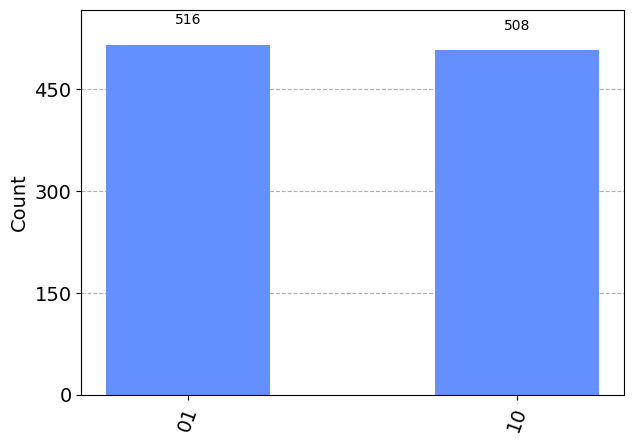
\includegraphics[width = .5\textwidth]{scrn-2024-01-03-09-40-24.png}
    \caption{Results from the code shown above.}
\end{figure}
\section*{Quantum Teleportation}
The Bell basis is defined as
\begin{align*}
\ket{\Phi_1} &= \frac{\ket{00} + \ket{11}}{\sqrt{2}} & \ket{\Phi_2} &= \frac{\ket{00} - \ket{11}}{\sqrt{2}} \\
\ket{\Phi_3} &= \frac{\ket{01} + \ket{10}}{\sqrt{2}} & \ket{\Phi_4} &= \frac{\ket{01} - \ket{10}}{\sqrt{2}}
\end{align*}
\begin{itemize}
    \item[(a)] Consider the state $\ket{\phi} = \ket{\psi}\ket{\Phi_1}$, where $\ket{\psi} = \alpha \ket{0}+ \beta\ket{1}$ is any 1-qubit state. If a measurement is made in the Bell basis and the outcome $i$ is observed, then the system is left in the state $\frac{1}{N}(\ketbra{\Phi_i}{\Phi_i}\otimes I) \ket{\phi}$, where the factor of $\frac{1}{N}$ just normalizes the resulting state. Say the outcome $i=1$ is measured. In what state does this leave the system?
    \item[(b)] We have previously shown that $XI\ket{\Phi_1} = \ket{\Phi_3}$, $YI\ket{\Phi_1} = -i\ket{\Phi_4}$, and $ZI\ket{\Phi_1} = \ket{\Phi_2}$. Using this, if any outcome $1 \leq i \leq 4$ is measured, what state is the system left in? 
\end{itemize}

\subsection*{Solution}
\subsubsection*{Part a}
We begin by writing $\ket{\Phi_1} = \frac{1}{\sqrt{2}}\sum_{i}^2\ket{ii}$ for convenience. Then the projector above can be written $\ketbra{\Phi_1}{\Phi_1} = \frac{1}{2}\sum_{i,j}^2 \ketbra{ii}{jj}$. Similarly, we write $\ket{\psi} = \sum_{k}\psi_k \ket{k}$, where $\psi_1 = \alpha$ and $\psi_2 = \beta$. Applying this to the state $\ket{\psi}\ket{\Phi_1} = \sum_{kl}^2\psi_k\ket{kll}$. Then applying the projector, 
\begin{align*}
    (\ketbra{\Phi_i}{\Phi_i}\otimes I)\ket{\psi}\ket{\Phi_1} &= \qty(\frac{1}{2}\sum_{ij}\ketbra{ii}{jj}\otimes I)\frac{1}{\sqrt{2}}\sum_{kl}\psi_k\ket{kll} \\
    &= \frac{1}{\sqrt{2^3}}\sum_{ijkl}\psi_k \ket{ii} \braket{jj}{kl}\ket{l} \\
    &= \frac{1}{\sqrt{2^3}}\sum_{ijkl}\psi_k \ket{ii}\delta_{jk}\delta_{jl}\ket{l} \\
    &= \frac{1}{\sqrt{2^3}}\sum_{ij}\psi_j \ket{ii}\ket{j} \\
    &= \frac{1}{2}\ket{\Phi_1}\ket{\psi}
\end{align*}
This gives $N = 2$ and the resultant state is $\ket{\Phi_1}\ket{\psi}$. With this operation, we have successfully mapped the state $\ket{\psi}\ket{\Phi_1} \mapsto \ket{\Phi_1}\ket{\psi}$, which is quantum teleportation.

\subsubsection*{Part b}
Let $\ket{\Phi_i} = P_iI\ket{\Phi_1}$, where $P_1 = I$, $P_2 = Z$, $P_3 = X$, and $P_4 = Y$. A measurement in the Bell basis results in a value $i=1,\dots, 4$ corresponding to the measured Bell state. After measurement, the system is left in the state
\begin{equation}
    \qty(P_iI\ketbra{\Phi_1}{\Phi_1}P_iI \otimes I)\ket{\psi}\ket{\Phi_1} = P_iI\qty(\ketbra{\Phi_1}{\Phi_1} \otimes I)(P_i\ket{\psi})\ket{\Phi_1}
\end{equation}
All we have done is use associativity to change the parenthesis. The above equation is equivalent to teleporting the state $P_i\ket{\psi}$ and then applying $P_iI$, which leaves the system in the state
\begin{equation}
P_iI\ket{\Phi_1}P_i\ket{\psi} = \ket{\Phi_i}P_i\ket{\psi}
\end{equation}
Applying $P_i$ to the teleported qubit based on the measurement result to cancel the unwanted operator completes the teleportation algorithm.
\section*{Parity Measurements}
In outer product form,
$$
Z \otimes Z = (\ketbra{0}{0}-\ketbra{1}{1})\otimes (\ketbra{0}{0}-\ketbra{1}{1}) = (\ketbra{00}{00} + \ketbra{11}{11}) - (\ketbra{01}{01} + \ketbra{10}{10})
$$
Letting $P_{1} = \ketbra{00}{00} + \ketbra{11}{11}$ and $P_{-1} = \ketbra{01}{01} + \ketbra{10}{10}$, this can be simply written
$$
Z \otimes Z = P_{1} - P_{-1}
$$
This shows us that $Z \otimes Z$ has two eigenspaces, the first with eigenvalue $+1$ spanned by $\ket{00}, \ket{11}$ and the second with eigenvalue $-1$ spanned by $\ket{01}, \ket{10}$. The operators $P_1, P_{-1}$ are called projectors into each eigenspace, because they map anything in the respective eigenspace to itself and anything outside to zero. This is an example of degeneracy, meaning that there is more than one eigenvector for the same eigenvalue. In the degenerate case, measuring $Z \otimes Z$ and finding the outcome $i$ applies the projector $P_i$ to the system and then normalizes the state. The Borne rule for determining the measurement probabilities in the degenerate case is
$$
p_\psi(i) = \bra{\psi}P_i\ket{\psi}
$$

\begin{itemize}
\item[(a)] If the system is in the state $\ket{\psi} = \alpha \ket{00} + \beta \ket{11}$ and the outcome $+1$ is measured, what state is the system left in after? What about if the state is $\ket{\psi'} = \alpha \ket{10} + \beta\ket{01}$ and the outcome $-1$ is measured?
\item[(b)] Consider the state $\qty(\frac{I+iX}{\sqrt{2}}\otimes I)\ket{\psi}$. Upon measuring $Z \otimes Z$, what is the probability of seeing the outcome $+1$ and the outcome $-1$? In what state does this leave the system in either case?
\end{itemize}
\textit{Note: This is the most basic example of error detection. If the environment randomly applies $X$ to one of the qubits, then measuring the operator $Z \otimes Z$ will indicate that an error has occurred.}

\subsection*{Solution}

\subsubsection*{Part a}
We notice that $P_1\ket{00} = \ket{00}$ and $P_1\ket{11} = \ket{11}$ because both states have even bit parity, so $P_1 \ket{\psi} = \ket{\psi}$. An outcome of $+1$ corresponds to applying $P_1$ to $\ket{\psi}$ and then renormalizing the state. Applying $P_1$ to $\ket{\psi}$ leaves the state unchanged, so the state and the corresponding amplitudes $\alpha$ and $\beta$ are unaffected by the measurement. The same is true for measuring $-1$ from the state $\ket{\psi'} = \alpha \ket{10} + \beta\ket{01}$. Both $\ket{10}$ and $\ket{01}$ have odd parity, so $P_{-1}\ket{\psi'} = \ket{\psi'}$. This means that a measurement of $-1$ leaves the state unaffected. 
\par The interpretation of this behavior is that the result of measuring $Z \otimes Z$ only carries information about the parity of the qubit states. Information is lost due to the degeneracy in the eigenspace. This causes the state to collapse only partially upon measurement. Since measuring $+1$ cannot distinguish states with even parity, a linear combination of even-parity states will not collapse upon measurement. 

\subsubsection*{Part b}
Let
\begin{equation}
    \ket{\phi} = \qty(\frac{I+iX}{\sqrt{2}})\otimes I\ket{\psi} = \frac{1}{\sqrt{2}}\ket{\psi}+ \frac{i}{\sqrt{2}}\ket{\psi'}
\end{equation}
Therefore $P_1\ket{\phi} = \frac{1}{\sqrt{2}}\ket{\psi}$ and $P_{-1}\ket{\phi} = \frac{i}{\sqrt{2}}\ket{\psi'}$. We recognize that $\ket{\psi}, \ket{\psi'}$ are orthonormal. Using this, we have 
\begin{equation}
\bra{\phi}P_1\ket{\phi} = \frac{1}{\sqrt{2}}\qty(\bra{\psi} -i\bra{\psi'})\frac{1}{\sqrt{2}}\ket{\psi} = \frac{1}{2}
\end{equation}
The outcome $+1$ is measured with probability $1/2$, and the state the system is left in is $\ket{\psi}$. Similarly,
\begin{equation}
\bra{\phi}P_{-1}\ket{\phi} = \frac{1}{\sqrt{2}}\qty(\bra{\psi} -i\bra{\psi'})\frac{i}{\sqrt{2}}\ket{\psi'} = \frac{1}{2}
\end{equation}
The outcome $-1$ is measured with probability $1/2$, and the state the system is left in is $\ket{\psi'}$. This is a simple demonstration of error detection. If the gate $\qty(\frac{I+iX}{\sqrt{2}})$ represents an accidental over-rotation of the first qubit, then measuring $Z\otimes Z$ either fixes the error by collapsing the state in to $\psi$ or collapses into an error state $\ket{\psi'}$, with each result indicated by the eigenvalue obtained. This is not full error correction, since the single measurement result is not enough to uniquely determine the error, for instance, on which qubit the error ocurred. 
\end{document}
